\documentclass[12pt]{article} 

% Set page margins and size
\usepackage[papersize={8.5in,11in}, left=1in, top=1in, right=1in, bottom=1in]{geometry}

%\usepackage[landscape]{geometry}

\usepackage[english]{babel}         % Permite escribir en espanol
\usepackage[ansinew]{inputenc}      % Permite escribir en espanol
\usepackage{graphicx}               % Para insertar graficos
\usepackage{float, verbatim}        % Para manejar la ubicacion de graficos
\usepackage{verbatim}               % Para escribir codigos
\usepackage{psfrag}                 % Para escribir en los graficos
\usepackage{url}                    % Para escribir direcciones web
\usepackage{subfigure}                 % Para poner varias figuras en el mismo marco
\usepackage{hhline}                 % Para poner varias figuras en el mismo marco
\usepackage{longtable}              % Para que las tablas no se corten
\usepackage{cancel}
\usepackage{isorot}
\usepackage{caption}

\usepackage{amsmath}               
\usepackage{bm}
\usepackage{amsthm}                 
\usepackage{amssymb}                
\usepackage{lscape}

\usepackage{color}

% Hyperlinks
\usepackage{hyperref}


\parindent=0pt
% Increase paragraph spacing
\setlength{\parskip}{6pt}
\usepackage{setspace}

\usepackage{booktabs}
\usepackage[flushleft]{threeparttable}
%\usepackage{tablefootnote}

\newcommand{\bi}{\begin{itemize}}
\newcommand{\ei}{\end{itemize}}
\newcommand{\Rkplus}{\mathbb{R}^K_+}
\newcommand{\bee}{\begin{equation}}
\newcommand{\eee}{\end{equation}}

\newcommand{\be}{\begin{equation*}}
\newcommand{\ee}{\end{equation*}}


\newtheorem{mydef}{Definition}
\newtheorem{ex}{Example}
\newtheorem{lemma}{Lemma}[section]
\newtheorem{prop}{Proposition}
\newtheorem{corr}{Correlary}
\newtheorem{axiom}{Axiom}[section]
\newtheorem{thm}{Theorem}[section]
\newtheorem{remark}{Remark}[section]
%\pagenumbering{gobble}

\usepackage{pgf}
\usepackage{tikz}
\usetikzlibrary{trees,shapes,snakes,fit}

\newcommand\independent{\protect\mathpalette{\protect\independenT}{\perp}}
\def\independenT#1#2{\mathrel{\rlap{$#1#2$}\mkern2mu{#1#2}}}
\renewcommand{\vec}[1]{\mathbf{#1}}
\usepackage{enumerate}

\begin{document}
{\Large \bf Intermediate Macroeconomics Recitation 2}

Topics: Empirical fit of the production model, TFP differences (Jones 4.3-4.5), review of labor supply by calculus of variations.

%\tableofcontents
 \section{Analyzing the Production Model}
 
 
 %These come up for the first time in the context of the firm's optimal choice of labor and capital. Please feel free to talk about that case (or the household problem) even though I will also do this in lecture. There are notes from prior years on Dropbox. But I have also added a reading about this to the syllabus. This is chapter 14 of Simon and Blume (1994). It may be useful to go through stuff from this reading.
 %References: Simon and Blume, Chapter 14
 
We have solved for the general equilibrium of the production model in terms of Y, the total (aggregate) output. However, it is output \textit{per capita} that determines a country's welfare. 

\begin{mydef} $y = \frac{Y}{L}$ is the output per person. $k = \frac{K}{L}$ is the capital per person. \end{mydef}

Then plugging the two new variables, y and k, back into the previous equilibrium, 

\begin{equation*}
y^*=\frac{Y^*}{L^*}=\frac{{\bar{A}}{\bar{K}}^{1/3}{\bar{L}}^{2/3}}{\bar{L}}={\bar{A}\bar{k}^{1/3}}
\end{equation*}%

  
Output per person ($y$) is higher when (1) productivity ($A$) is higher, and (2) capital per person ($k$) is higher. Note that increasing capital per person leads to \textbf{diminishing returns}.

\subsection{Empirical Fit of the Production Model (Jones 4.3)}

\begin{equation*}
y^*={\bar{A}\bar{k}^{1/3}}
\end{equation*}%

This is an {\bf empirical implication} of the model.
{\bf Development accounting} is using this equation to try to account for differences in output across countries. 

{\bf Data} that we need to check this implication: 

(1) Output, Capital, Labor - can be measured 

(2) Technology - hard to measure 

Start with the assumption that all countries have the same level of technology ($A$ normalized to 1). We compare the output per person of country x with that of the U.S.:

\begin{equation*}
 \bar{A_{x}}={\bar{A}_{US}}=1
\end{equation*}

\begin{equation*}
\frac{y_{x}^*}{y_{US}^*}=\left(\frac{\bar{k_{x}}}{\bar{k}_{US}}\right)^{1/3}
\end{equation*}

\begin{figure}[H]
\caption{The Model's Prediction for Per Capita GDP (U.S.=1). Note: assuming no difference in productivity, the model predicts smaller differences in income across countries than we observe.}
\centering
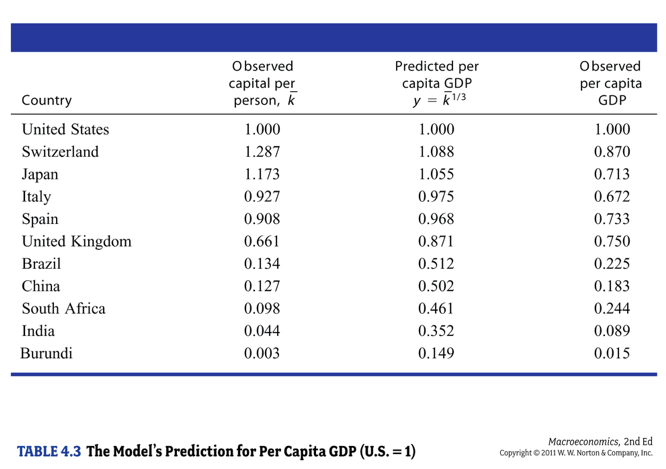
\includegraphics[width=120mm, scale=0.5]{Table_4-3.jpg}
\end{figure}

\begin{figure}[H]
\caption{Predicted Per Capita GDP in the Production Model}
\centering
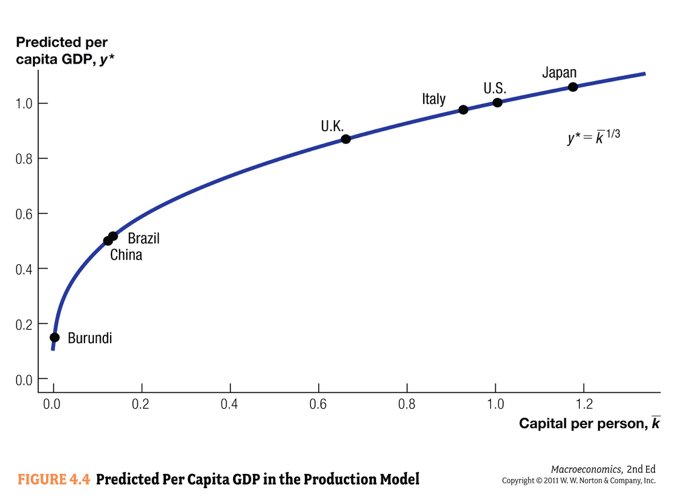
\includegraphics[width=120mm, scale=0.5]{Figure_4-4.png}
\end{figure}

\begin{figure}[H]
\caption{The Model's Prediction for Per Capita GDP (U.S.=1). Note: if the model prediction is successful, the data points should line up close to the 45-degree line.}
\centering
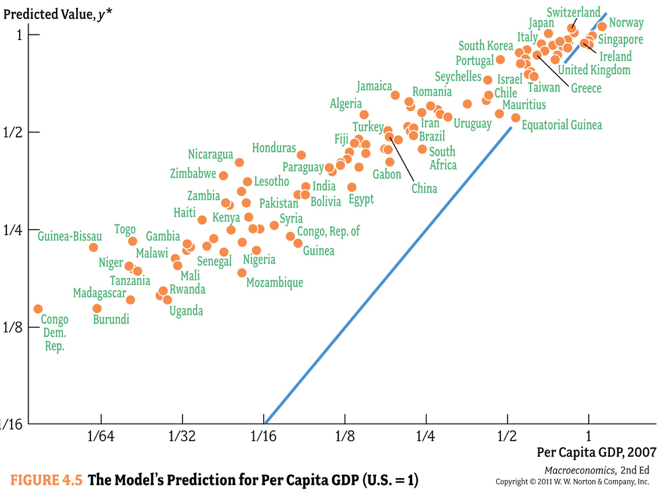
\includegraphics[width=120mm, scale=0.5]{Figure_4-5.png}
\end{figure}


The model gets the direction right: Poor countries produce less than their capital stocks. However, it systematically predicts countries to be richer than they actually are.

Possible reasons for the bad fit: 

(1) Mismeasurement in output, capital, labor

(2) Assumptions of model might be wrong: Functional form of production function; Skilled vs. unskilled labor; Some critical inputs might be missing (O-ring Theory) etc. 

We also assumed that countries have the same level of technology. To improve the fit of the model, we should develop a model to adjust for the differences in technology among countries.

\textbf{Optional}: Why doesn't capital flow from rich to poor countries? (Jones 4.3 Case Study)

\section{Total Factor Productivity (TFP) Differences}

Technology can be broadly interpreted as the \textbf{efficiency of production}. One limitation is that we don not have independent measure of the TFP. However, we have data on $y$ and $k$ for each country. Assuming the model is correct, we can calculate the level of TFP for each country that makes the model fit exactly.

Taking the ratio of TFPs for two different countries allows a further break down on what technology consists of,

\begin{equation*}
 \frac{A_{x}}{A_{US}}=\left(\frac{\frac{y_{x}}{y_{US}}}{\frac{k_{x}}{k_{US}}}\right)^{1/3}
\end{equation*}%

\subsection{Taking the Model to Data (Jones 4.3)}

\begin{figure}[H]
\caption{Measuring TFP so the Model Fits Exactly. Note: in order for the model to match the data, poor countries must be very inefficient in production, i.e. they have low TFP.}
\centering
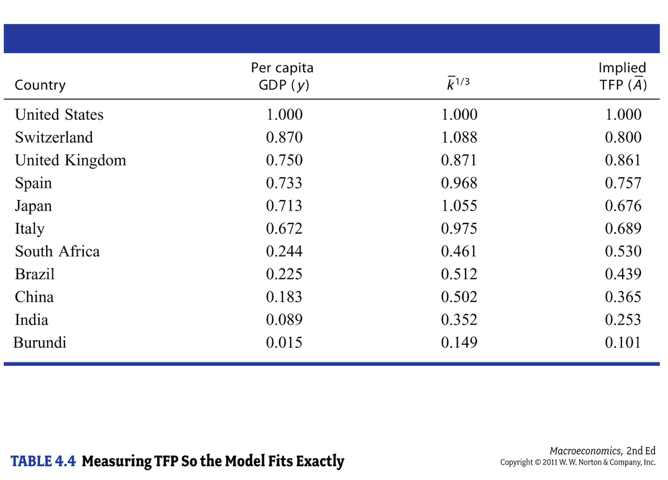
\includegraphics[width=120mm, scale=0.5]{Table_4-4.png}
\end{figure}

\begin{figure}[H]
\caption{Measuring TFP so the Model Fits Exactly}
\centering
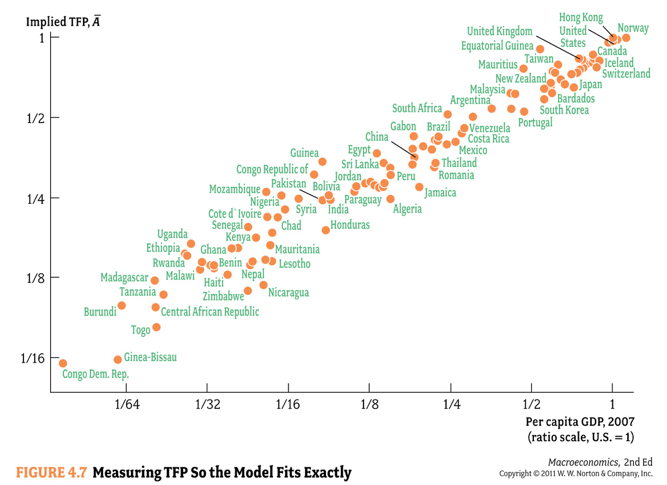
\includegraphics[width=120mm, scale=0.5]{Figure_4-7.png}
\end{figure}  

\textbf{Observations:}

(1) TFP differences can be up to a factor of 10 among countries.

(2) Both differences in TFP and differences in capital per capita explain the differences in per capita GDP. We can do an accounting exercise to determine the relative importance of these two factors.

\subsection{Explanations of TFP}

(1) Human Capital (education)

(2) Technology

(3) Institutions

(4) Misallocation

\section{Deriving Labor Supply by Calculus of Variations}

(Refer to Lecture Slides) The household chooses $H$, the hours worked (labor supply), to maximize the following utility function, 


\begin{equation*}\tag{1}
U({wH}^*) - V ({H}^*) 
\end{equation*}%

If the households adds or subtracts the labor supply by a small amount $\epsilon$, the new utility function is:

\begin{equation*}\tag{2}
U({w({H}^*+\epsilon)}) - V ({({H}^*+\epsilon)}) 
\end{equation*}%

If the maximum is achieved at ${H}^*$, then changing it to ${H}^*+\epsilon$ should not increase the value of the utility function, 
\begin{equation*}\tag{3}
(1) \ge (2) 
\end{equation*}%

Recall the Taylor series approximation, 
\begin{equation*}
f(x)=f(x_{0})+f^{\prime }(x_{0})(x-x_{0})+\frac{1}{2}f^{\prime \prime
}(x_{0})(x-x_{0})^{2}+...
\end{equation*}%

Or:

\begin{equation*}
f(x)=f(x_{0})+f^{\prime }(x_{0})(x-x_{0})+o(x-x_{0})
\end{equation*}%

,where all terms after the second term are replace with an error function, $o(x-x_{0})$. Then (2) can be rewritten as, 

\begin{equation*}\tag{4}
U({wH}^*) - V ({H}^*) + (U^{\prime}({wH}^*)w - V^{\prime} ({H}^*))\epsilon + o(\epsilon)
\end{equation*}%

$(1) \ge (4)$ gives:
\begin{equation*}
U({wH}^*) - V ({H}^*) \ge U({wH}^*) - V ({H}^*) + (U^{\prime}({wH}^*)w - V^{\prime} ({H}^*))\epsilon + o(\epsilon)
\end{equation*}%

\begin{equation*}
\Rightarrow (U^{\prime}({wH}^*)w - V^{\prime} ({H}^*))\epsilon \leq 0
\end{equation*}%

This is true for all values of $\epsilon$, so it must be that 
\begin{equation*}\tag{5}
U^{\prime}({wH}^*)w - V^{\prime} ({H}^*) = 0 
\end{equation*}%

${wH} = C$, so rearranging gets us to the same supply curve that we  derived previously, 
\begin{equation*}\tag{6}
\frac{V^{\prime} ({H}^*)}{U^{\prime}({C}^*)} = w
\end{equation*}

The intuition behind (6) is that, say $\epsilon>0$, the marginal benefit from increasing labor supply by $\epsilon$ is $U^{\prime}({C}^*)w\epsilon$, while the marginal cost is $V^{\prime} ({H}^*)\epsilon$. At the optimum, the two terms have to be equal, which gives us (6). 

\vspace{5mm}

What is the effect of a wage increase on labor supply? 
Review the {\bf substitution effect} and the {\bf income effect}. 


\end{document}
